\documentclass[a4paper]{article}

%% Language and font encodings
\usepackage[english]{babel}
\usepackage[utf8x]{inputenc}
\usepackage[T1]{fontenc}
%% Sets page size and margins
\usepackage[a4paper,top=3cm,bottom=2cm,left=3cm,right=3cm,marginparwidth=1.75cm]{geometry}

%% Useful packages
\usepackage{amsmath}
\usepackage{graphicx}
\usepackage[colorinlistoftodos]{todonotes}
\usepackage[colorlinks=true, allcolors=blue]{hyperref}
\usepackage{booktabs}
\usepackage{float}
\usepackage{siunitx}
\sisetup{output-exponent-marker=\ensuremath{\mathrm{e}}}

\title{Heuristic Optimization : Implementation exercise 2}
\date{May 17, 2017}
\author{Nikita Marchant (nimarcha@vub.ac.be)}

\setlength{\parskip}{7pt}%
\setlength{\parindent}{0pt}%
\renewcommand{\baselinestretch}{1}

\begin{document}
\maketitle

\section{Introduction}

This document is the report of the implementation exercise 2 for the Heuristic Optimization course.
The exercise asks to implement two stochastic local search algorithms for the the permutation flow-shop problem with the sum weighted completion time objective (also called PFSP-WCT).

The PFSP-WCT has not been thoroughly studied in the literature so i used some inspiration from papers studying the PFSP with flowtime that is more studied.

\section{Algorithms}

The first algorithm is an Iterated Local Search (ILS) inspired from \cite{panruiz2012} and the second is a genetic algorithm inspired from \cite{zhang2009}.

\subsection{Iterated Local Search}

The Iterated Local Search is a stochastic meta-heuristic
known to be applicable to multiple optimization problems~\cite{Lourenco2010}.

It consists of these steps :

\begin{enumerate}
    \item Generate an initial solution
    \item Apply a local search to the solution
    \item When stuck in a local optimum, apply a perturbation
    \item Apply a local search to the solution
    \item Use an acceptance criterion for the perturbed then optimized solution
    \item Go back to 3 or stop when a termination criterion is met.
\end{enumerate}

\subsubsection{Initialization method: $LR(x)$}
\label{LR}

The initialization method used in this implementation and in \cite{panruiz2012} is the $LR(x)$ heuristic introduced by \cite{liu2001}.  It consist in three steps :
\begin{enumerate}
    \item Rank the jobs by their weighed sum of flowtime
    \item Generate $x$ solutions by inserting the job from position $x$ at the front of the solution
    \item Select the sequence with the minimum weighted flow time
\end{enumerate}

\subsubsection{Local search}
\label{RZ}
The local search that was implemented is the iterated RZ (IRZ). The RZ uses a insertion neighborhood.
It sequentially inserts each job at each possible position in the candidate solution (thus is in $O(n^2)$ complexity if $n$ is the number of jobs) and keeps the best one.

The IRZ applies RZ until a local optimal solution is found (i.e. the RZ does not yield a better result).

\subsubsection{Perturbation method}
\label{pertu}

After finding a local optimum, a perturbation is applied to be able to escape the local optimum and extend the search space.

The perturbation method consists of $\gamma$ random insertion moves : each move selects randomly a job and moves it to a random position.

\subsubsection{Acceptance criterion}

After finding a local optimum, we have to decide if we keep the solution. I chose to implement the {simulated annealing} as the criterion with $\lambda \cdot \frac{\sum_{j=1}^{n} \sum_{i=1}^{m} p_{ij}}{10 min}$ as a constant temperature.

\subsubsection{Termination criterion}

For both algorithm, the termination criterion is the time. For instances of size $N=50$, i stop at 70 seconds and for $N=100$ i stop at 200 seconds. Theses values were chosen as 100 times the runtime of the algorithms implemented in the first part.


\subsection{Genetic algorithm}

My implementation of a genetic algorithm is inspired form \cite{zhang2009} with some slight differences.

\begin{enumerate}
    \item Generate a initial population
    \item Generate a new generation with the crossover operator
    \item Perturbate each chromosome with a given probability
    \item Apply a local search on each chromosome
    \item Merge the old and the new population and select the eligible chromosomes to be kept
    \item Goto 2 or stop if the termination criterion is met
\end{enumerate}

\subsubsection{Generation of the initial population}

The initial population consists of one chromosome generated with $LR(x)$ (see \ref{LR}) and the other
are generated as random permutation of the job set.

\subsubsection{Crossover operator}

Two crossover operators were implemented, both described in \cite{zhang2009}. SJOX and its improvement with an artificial chromosome generated by WSMGS (weighted simple mining gene structure). The latter was used for the result section.


\subsubsection{Mutation operator}

The mutation operator is the same as in \ref{pertu} but applied only with $P_m \cdot \sqrt{U + 1}$ probability.
$U$ is defined as the number of generation since the last improvement to the global solution. This is not present in \cite{zhang2009} but helps to unstuck the algorithm when it is stuck in a local optimum since a long time.


\subsubsection{Local search}

The local search method is RZ (as explained in \ref{RZ}) but also has an original addition, if $U$ is bigger than $U_{IRZ}$, a IRZ algorithm is used instead because the mutation rate is much higher so the chromosome is highly perturbed.

Using a IRZ all the time was tried but yielded no better results and was significantly slower\footnote{Due to the lack of computing power (see \ref{power}), this hypothesis could not be formally proved.}.

\subsubsection{Population selection}

When selecting the population, many methods were tried : the best, uniform and roulette methods.

These methods were extracted from \cite{Kouki}. They conclude that the uniform method is superior for problems on PFSP of our size but during my experiments, it seemed that the method \textit{best} was superior\footnote{Again, due to a lack of computing power, this could not be proved}.

The \textit{best} method selects the $N$ best chromosomes form the concatenation of parents and children.


\section{Parameters}

The parameters cited above were fixed empirically or taken from the literature because of computation power issues (see \ref{power}). Here are the values fixed in the implementation :

\begin{itemize}
    \item $N$ (population size): 50 (taken directly from \cite{zhang2009})
    \item $U_{IRZ}$: 5
    \item $P_m$ (mutation rate): $0.02$
    \item $E$ (number of elites): $5$
    \item $x$ (from $LR(x)$): $\frac{m}{n}$ (the number of jobs divided by the number of machines) (taken directly from \cite{panruiz2012})
    \item $\gamma$ (number of random moves) : 4
    \item $\lambda$ (temperature parameter): 4
\end{itemize}

\subsection{Computation power limitation}
\label{power}

A big road-blocker for finding the optimal parameters of choosing a method over another was the limitation by the available computing power. As the exercise suggests running at least each instance 5 times for 200 seconds, the run time is over 16 hour per method or parameter on one CPU.

This meant that some choices were made relying solely on the literature (that was most of the time studying PFSP and not PFSP-WCT) or a few tests on a few instances without any statistical study due to the lack of data.

The final runs made for the result section were ran on two 32-CPU virtual machines in the cloud to be able to (re-)produce them in time because running experiments for 32 continuous hours on my laptop was not feasible.

\section{Results}

For the exercise, two experiments were ran. The first was a run of both algorithms five times on each instance.
The second was a run of both algorithms, 25 times on the first 5 instances of size 5 with a cutoff time 10 times bigger.


\subsection{Score}

\subsection{Average percentage deviation}

        \begin{figure}[H]
            \centering
            \label{dev_algo_instance}
            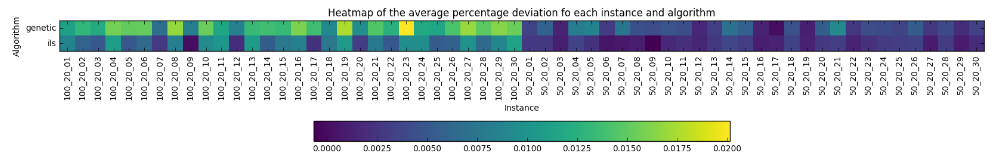
\includegraphics[width=1.1\textwidth]{heatmap.png}
            \caption{Average percentage deviation from best known solutions for each instance and algorithm}
        \end{figure}

In this heatmap, we can clearly see that my algorithms perform better on the instances of size 50 than size 100. This might be because the time termination criterion is too low for the instances of size 100. It also seems that ILS is better than the genetic on instances for size 100.

        \begin{figure}[H]
            \centering
            \label{dev}
            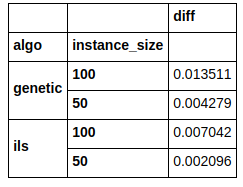
\includegraphics[width=0.3\textwidth]{dev.png}
            \caption{Average percentage deviation from best known solutions for and algorithm}
        \end{figure}

By looking at the average percentage deviation in the Figure 2, it seems that ILS is better for both sizes.

        \begin{figure}[H]
            \centering
            \label{corr}
            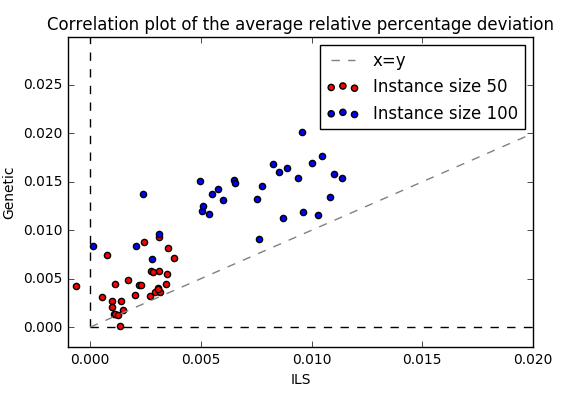
\includegraphics[width=0.8\textwidth]{corr.png}
            \caption{Average percentage deviation from best known solutions for and algorithm}
        \end{figure}

We can then make a correlation plot of the same data to visualize the distribution. We can see that almost every point is above $x=y$ thus, that ILS was better than genetic almost every time.

To be sure of this assumption, we can use statistical tests to verify this hypothesis. The metric used is the Wilcoxon test with the null hypothesis that both samples are drawn from the same distribution.

For the instances of size 50, the p-value is \num{6.33e-06} and for the size 100, \num{1.73e-06}. Both are bigger than 0.5 thus the hypothesis is rejected. This means that ILS is significantly better than genetic on both instance sizes.

\subsection{Run times}

After comparing the scores of both algorithms, we can compare the run times before finding a solution close enough to the best known solution. Theses graphs show the distribution of the time needed per algorithm and per allowed deviation.

Unfortunately, those graphs are not representative because some instances did not find an acceptable solution before the timeout. For the 0.05\% deviation the genetic algorithm was not able to find a acceptable solution for 20 instances out of 125. For the 0.01\% deviation, the ILS missed 46 instances and the genetic 56.

The bar charts just ignore those missing instances and thus do not have the same amount of points.

These charts seem to show that ILS is faster to find acceptable solutions for each tolerance. (And the count of missing instances too).

We can confirm this with Wilcoxon tests: they all reject the null hypothesis with p-values of \num{2.96e-22}, \num{6.87e-22}, \num{7.22e-19} and \num{6.07e-17}.


        \begin{figure}[H]
            \centering
            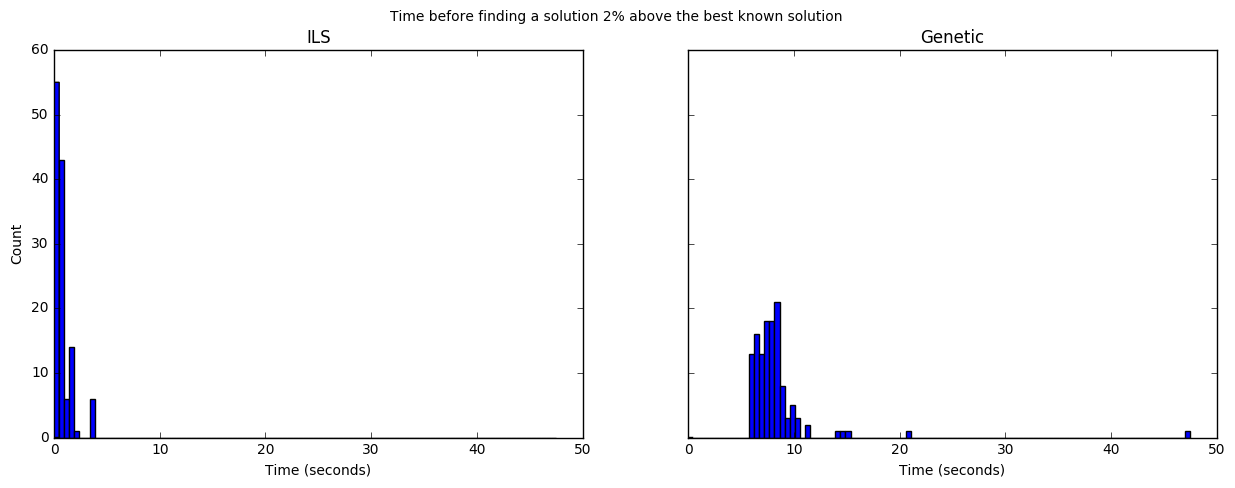
\includegraphics[width=\textwidth]{t2.png}
        \end{figure}
                \begin{figure}[H]
            \centering
            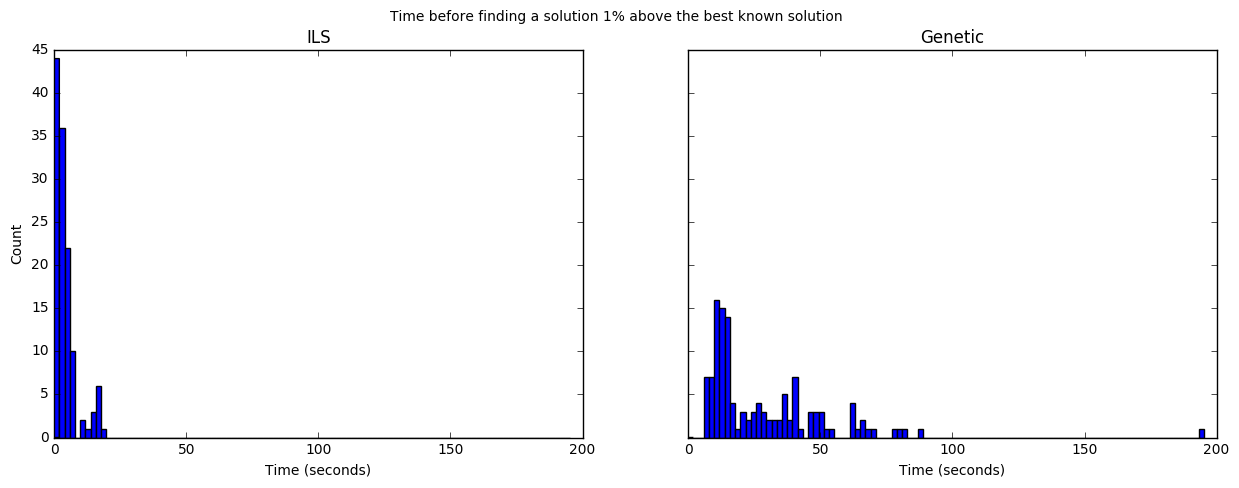
\includegraphics[width=\textwidth]{t1.png}
        \end{figure}
                \begin{figure}[H]
            \centering
            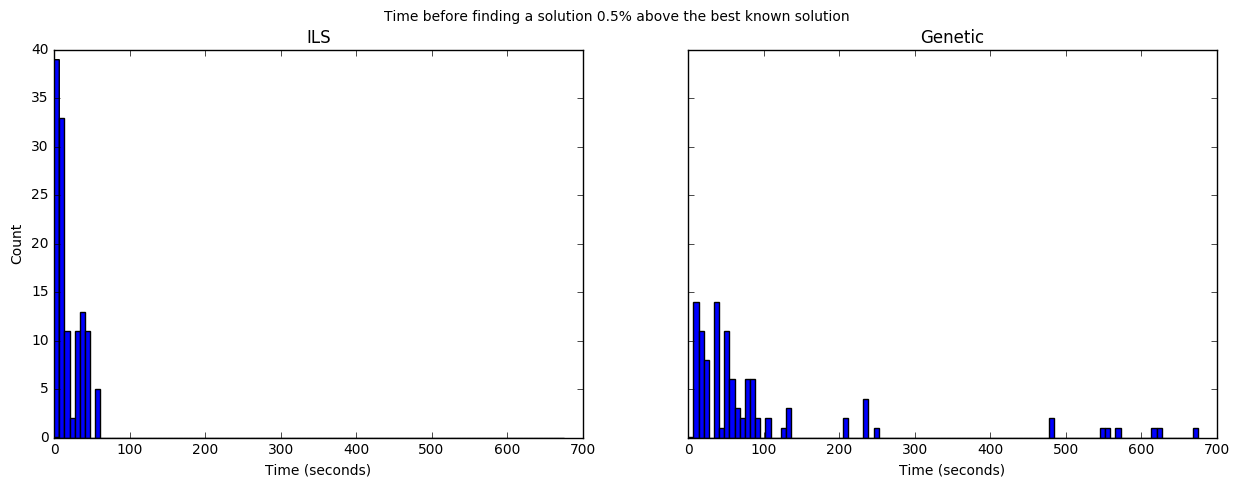
\includegraphics[width=\textwidth]{t05.png}
        \end{figure}
                \begin{figure}[H]
            \centering
            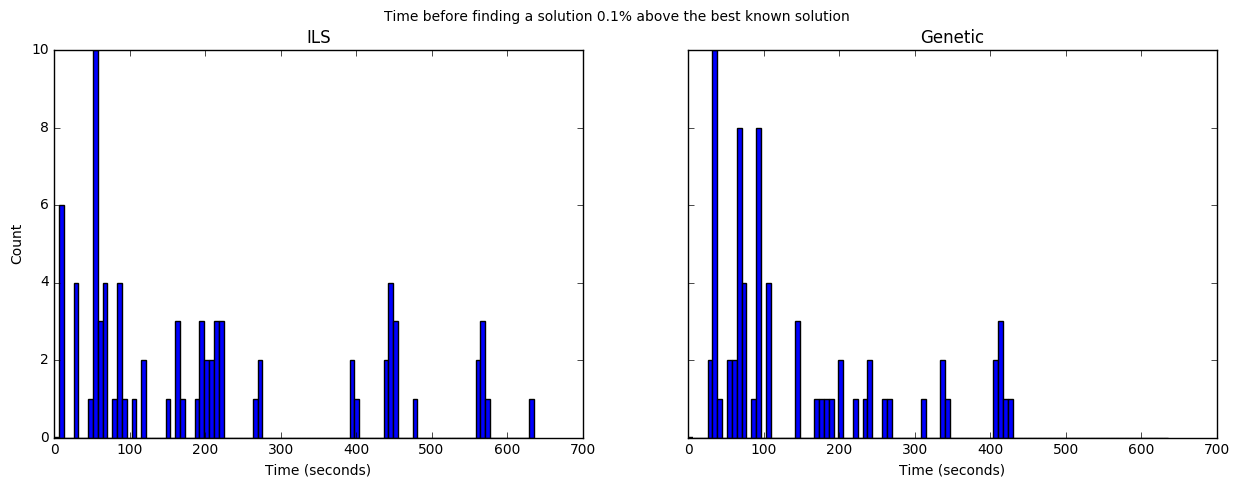
\includegraphics[width=\textwidth]{t01.png}
        \end{figure}

\section{Implementation}

The implementation is written in C++17 and uses only the standard library. It can be compiled with \texttt{make} and ran with \texttt{./fssp \textit{instance\_path timeout algorithm}} where \texttt{\textit{instance\_path}} is the UNIX path to the instance, \texttt{\textit{timeout}} is the timeout for the termination criterion in seconds and \texttt{\textit{algorithm}} is \texttt{ils} or \texttt{genetic}.
Example : \texttt{./fssp instances/100\_20\_28 200 ils}.

It outputs the score of the initial solution. Then for each generation or improvement, it outputs the time elapsed in seconds and the intermediate score. The last line is the best achieved score for the run.

The implementation was based on the one from the previous exercise and thus still contains old code, not used anymore.


\bibliographystyle{apalike}
\bibliography{bib}

\end{document}
